\documentclass[a4paper,11pt]{article}

\usepackage[a4paper,margin=1in]{geometry}
\usepackage[utf8]{inputenc}
\usepackage{amsmath}
\usepackage{amssymb}
\usepackage{amsthm}
\usepackage{booktabs}
\usepackage[small]{caption}
\usepackage{cite}
\usepackage{colortbl}
\usepackage{enumitem}
\usepackage{framed}
\usepackage{graphicx}
\usepackage{multirow}
\usepackage{microtype}
\usepackage[dvipsnames]{xcolor}
\usepackage[unicode]{hyperref}
\usepackage{amsfonts}
\usepackage{algorithm}
\usepackage{algpseudocode}
\usepackage{bm}
\usepackage{mathtools}
\usepackage{subcaption}

\usepackage{listings} % replace with nice syntax hl

\bibliographystyle{plainurl}

\setlength{\OuterFrameSep}{0.3ex}
\setlength{\FrameSep}{1.5ex}

\newcommand{\myaff}[1]{\,$\cdot$\, {\small #1}\par\smallskip}
\newcommand{\fakeparagraph}[2]{\par\noindent\textbf{#1}\hspace{1em}#2}

\usepackage{thm-restate}
\usepackage{cite}

% Problem definition environment
\newfloat{problemdef}{htbp}{loa}
\floatname{problemdef}{Problem}
\newcommand{\problemcaptionkludge}{\rule[-.3\baselineskip]{0pt}{\baselineskip}}

\theoremstyle{plain}
\newtheorem{theorem}{Theorem}[section]
\newtheorem{lemma}[theorem]{Lemma}
\newtheorem{corollary}[theorem]{Corollary}
\newtheorem{observation}[theorem]{Observation}
\theoremstyle{definition}
\newtheorem{definition}[theorem]{Definition}
\newtheorem{example}[theorem]{Example}
\theoremstyle{remark}
\newtheorem*{remark}{Remark}
\newtheorem{openquestion}[theorem]{Open question}

\newcommand{\tcode}[1]{\texttt{#1}}
\newcommand{\tperm}[1]{\texttt{#1}}
\newcommand{\tsub}[1]{\textsubscript{#1}}

% Well-parenthesized commands
\newcommand{\set}[1]{\ensuremath{\left\{#1\right\}}}

\newenvironment{myabstract}
{\list{}{\listparindent 1.5em%
        \itemindent    \listparindent
        \leftmargin    0cm
        \rightmargin   0cm
        \parsep        0pt}%
    \item\relax}
{\endlist}

\newenvironment{mycover}
{\list{}{\listparindent 0pt
        \itemindent    \listparindent
        \leftmargin    0cm
        \rightmargin   0cm
        \parsep        0pt}%
    \raggedright
    \item\relax}
{\endlist}

\begin{document}

\begin{mycover}
{\huge\bfseries\boldmath Tree Borrows\par}
\bigskip
\bigskip
\bigskip


Author: \textbf{Neven Villani}
\myaff{ENS Paris-Saclay}

~\newline

Advisor: \textbf{Derek Dreyer}
\myaff{MPI for Software Systems}


Advisor: \textbf{Ralf Jung}
\myaff{ETH Zürich}


\end{mycover}
\medskip

\begin{myabstract}
\fakeparagraph{Abstract.}
\end{myabstract}
\medskip


\section{Introduction}

While the purpose of type systems and typing information in programs is usually
presented as primarily a matter of security (strict type systems can rule out
at compilation-time a number of bugs), they also enable compilers to generate
more efficient code in both space and time. Languages with strict compile-time
type systems can avoid the need for typing metadata at runtime, have fewer
bounds checks for memory accesses, or even in the case of Rust eliminate the
need for a runtime garbage collector entirely.

In Rust the type system includes aliasing information (mutability and uniqueness),
which is to be used not only for safety guarantees, but also to improve
performance and enable optimizations that are only valid under certain aliasing
guarantees.
We aim to define formally what these aliasing guarantees are for Rust, as
well as show how to check them and use them in proving the validity of compiler
optimizations.

\subsection{Motivating example}

As a first concrete example, consider the following function:
\begin{lstlisting}
fn example1(x: &mut u64, y: &mut u64) -> u64 {
     let xval = *x; // First read of *x
     *y = xval + 1;
     let xval = *x; // Second (redundant ?) read of *x
     return xval;
}
\end{lstlisting}

Because mutable references in Rust are required to be unique, \tcode{x} and
\tcode{y} must point to disjoint regions of memory. In particular the
instruction \tcode{*y = xval + 1} constitutes a write to \tcode{y}, but it
cannot affect the memory covered by \tcode{x}: the value \tcode{*x} is unaffected
and thus the second read of \tcode{*x} is redundant. This function can be
optimized to perform one fewer operation by deleting the second line on which
\tcode{*x} is read, without modifying behavior.

Unfortunately there is a huge gap in the proof above: we have not specified
by whom, in what contexts or in which manner mutable references are ``required''
to be unique. This is the purpose of Tree Borrows.

Indeed there exists in Rust the \tcode{unsafe} keywords which
allows the programmer to bypass certain compiler checks by extending their
available instruction set: among other things the \tcode{unsafe} keyword allows
dereferencing raw pointers in the following manner:
\begin{lstlisting}
fn context1() {
    let mut data = 42u64;
    let data_ptr = &mut data as *mut u64;
    let x: &mut u64 = unsafe { &mut *data_ptr };
    let y: &mut u64 = unsafe { &mut *data_ptr };
    let result = example1(x, y);
    assert!(result == 43);
}
\end{lstlisting}
Here we use \tcode{unsafe} instructions to obtain two mutable references
to the same location, and we pass both of them to \tcode{example1}.
While in this context the original version of \tcode{example1} will return
\tcode{43}, the optimized version will instead return \tcode{42}.

The optimization shown here is thus not unconditionally valid: violating the
unicity requirement of mutable references has enabled us to create a program
in which the optimization does not preserve behavior.

However we want this optimization to be valid, on the grounds of \tcode{context1}
being a ``bad'' program that violates some assumptions that we want to be able
to make. This issue is solved by adjusting the operational semantics of Rust
in a way that declares \tcode{context1} ``Undefined Behavior'' (UB):
a program exhibits UB when it performs some forbidden instruction.
Compilers can assume that programs do not exhibit UB, and optimizations are
not required to preserve the observable behavior of such programs.

There is a tradeoff in what programs can be declared UB, indeed for compiler writers
the more programs are declared UB the more powerful optimizations can be made and
the more freedom there is in what is considered a correct compiler, while for language
users the more programs are declared UB the less the execution closely matches the source
code. Consider for example the two extreme cases:
\begin{itemize}
    \item if all programs are UB then it is valid to compile all programs as an
        empty sequence of instructions, optimizations are too powerful and the language
        is so underspecified as to become useless;
    \item on the other hand if no program is UB, then few to no optimizations are possible.
\end{itemize}
Both sides however have an interest in the rules governing UB being clear and well-defined:
if the rules are vague then compiler writers are unsure what assumptions they can make,
and language users may accidentally write a program that exhibits UB.

An explicit design decision of Rust is that programs that that do not use the
\tcode{unsafe} keyword cannot be declared UB. For \tcode{unsafe} to be useful,
it should also hold that it is not too difficult to write unsafe Rust that is not
UB. Tree Borrows should thus:
\begin{itemize}
    \item \textbf{Declare enough programs UB that some useful optimizations are valid.}
        We evaluate Tree Borrows on this aspect by providing proofs of validity of such
        optimizations using the aliasing assumptions allowed by the Tree Borrows semantics.
    \item \textbf{Declare as little UB as possible in programs that have already been written.}
        Each program retroactively declared to exhibit UB is a violation of backwards compatibility,
        we must ensure that these are few and justifiable.
        To check this aspect we implement the Tree Borrows semantics in the Miri
        interpreter and run the OS-independent part of the Rust standard library
        test suite using this semantics. We found very few rejected instances, and
        the suggested changes were accepted and merged back into the standard library.
    \item \textbf{Have rules that are simple, consistent and intuitive.}
        While it is difficult to measure this objectively, we argue that compared
        to its predecessor Stacked Borrows, Tree Borrows is more consistent in
        its handling of pointers. In particular a number of bug reports on the
        Github page of Miri show that users misunderstand some details of the
        behavior of Stacked Borrows, and we have ensured that such misunderstandings
        are not present in Tree Borrows.
    \item \textbf{Be efficient.} In addition to being humanly understandable, Tree Borrows
        should also be verifiable in practice without too much overhead in Miri.
        We compare it to benchmarks of Stacked Borrows and observe a noticeable slowdown,
        but not to the point that it would be an obstacle to the usability of Miri.
\end{itemize}

\section{Aliasing in Rust}

In this section we explain the features of Rust that we are interacting with --
mostly the different kinds of pointers available -- and provide an intuition
for the aliasing constraints they should satisfy.

We call ``safe Rust'' the subset of the complete Rust language (more explicitly called ``unsafe Rust'')
that does not use the \tcode{unsafe} keyword (and thus does not use any \texttt{unsafe}
instructions).

\subsection{References and raw pointers}

Rust offers a kind of pointer with more guarantees than its counterpart in most
languages: references. Written \tcode{\&} (\texttt{let x:~\&T = \&t;}) or
\tcode{\&mut} (\texttt{let x:~\&mut T = \&mut t;}) for immutable and mutable
references respectively.

These references should satisfy ``aliasing XOR mutability'': for a given memory
location, if a mutable reference exists there cannot also be other mutable or
immutable references. We can have access to either unique write permissions or
shared read permissions, not both.


As a means of interfacing with C code and expressing complex pointer manipulations,
Rust also offers another type of pointers, called raw pointers, written
\tcode{*const T} for immutable raw pointers and \tcode{*mut T} for mutable
raw pointers. There pointers can bypass some requirements of references (there
can exist multiple \texttt{*mut T} to the same location), but their use is more
dangerous and dereferencing raw pointers can be done only in blocks marked by
the keyword \tcode{unsafe \{...\}} thus their use is usually restricted to
situations where they are absolutely necessary.
Several \tcode{*mut T} can exist simultaneously.


The following snippet shows some conversions between these kinds of pointers:
\begin{lstlisting}
let mut data = 42u64;
let some_mut_ref: &mut u64 = &mut data;
let const_from_mut: &u64 = &*some_mut_ref;
let reborrow_mut: &mut u64 = &mut *some_mut_ref;
let mut_ptr: *mut u64 = &mut *some_mut_ref as *mut u64;
let ref_from_ptr: &mut u64 = unsafe { &mut *mut_ptr };
\end{lstlisting}

\section{Limitations of existing tools}

\subsection{The Borrow Checker}

The Borrow Checker is a compile-time verification of some aliasing rules, and
in the presence of safe Rust it is able to guarantee that mutable references
have exclusive access and that shared references have access to data that will
not be mutated. However it is in several aspects not fine-grained enough compared
to the model we want to develop.

We show here that there are both places where strictly adhering to the behavior
of the Borrow Checker would lead to too little UB and others where there would
be too much UB.

However in places where Tree Borrows does not follow the same rules as the
Borrow Checker the following should always hold: code that does not use
\tcode{unsafe} \textit{and} is accepted by the Borrow Checker should never
be UB.

\paragraph*{Bypassing the Borrow Checker with \texttt{unsafe} code.}
The Borrow Checker does not track borrows for raw pointers, so the easiest
--- but usually incorrect --- way to resolve compilation errors raised by the
Borrow Checker is to insert round trips to cast references to and from raw
pointers as follows
\begin{lstlisting}
// Rejected by the Borrow Checker.
// Expected to be UB.
fn alternate_writes() {
    let x = &mut 0u64;
    let y = &mut *x;
    let z = &mut *x;
    *y += 1;
    *z += 1;
}

// Accepted by the Borrow Checker.
// Expected to be UB.
fn alternate_writes_raw() {
    let x = &mut 0u64;
    let y = unsafe { &mut *(x as *mut u64) };
    let z = unsafe { &mut *(x as *mut u64) };
    *y += 1;
    *z += 1;
}
\end{lstlisting}

Since the explicit purpose of Tree Borrows is to also verify and optimize
\tcode{unsafe} code, it should be more robust than this. This is both so that
\tcode{unsafe} code actually gets checked and so that the use of \tcode{unsafe}
does not completely block all optimizations.

\paragraph*{Borrow conflicts undecidable at compile-time.}
As we have shown in \tcode{example1} above, whether a function call triggers
UB is in general dependent on what arguments it receives at runtime. Since the
usual reason that \tcode{unsafe} code is used in the first place is usually
that its safety relies on properties undecideable at compile-time, we define
UB at runtime. If some piece of code is unreachable then it cannot produce UB.

This is however not true of the Borrow Checker, which has to operate at compile-time,
as shown by the following example
\begin{lstlisting}
// Rejected by the Borrow Checker.
// Expected to not be UB.
fn unreachable_borrow() {
    let x = &mut 0u64;
    let y = &mut *x;
    if false {
        let z = &mut *x;
        *z += 1;
    }
    *y += 1;
}
\end{lstlisting}

\subsection{Stacked Borrows}

Stacked Borrows already adresses the two issues we have raised above with
why the Borrow Checker is insufficient: it executes at runtime and it handles
\tcode{unsafe} code as well. There are however a few aspects in which
Stacked Borrows behaves in ways that are too strict or too unpredictable.

\paragraph*{Reads should not invalidate other reads.}
An optimization that should always be possible is to permute two adjacent and independent
read accesses. Since a read access cannot alter the outcome of another, permuting
two reads produces a program that is guaranteed to have the same outcome.

Unfortunately that is not an optimization that Stacked Borrows always allows
because under some circumstances permuting two adjacent reads can introduce new
UB that was not in the original program, and of course introducing UB in a program
that did not contain any is not a valid optimization.

Thus of the two following functions, in which the only difference is a reordering
of read-only accesses, only one is UB and replacing the other with it is not
a valid program transformation.
\begin{lstlisting}
// UB according to Stacked Borrows.
fn read_xy() {
    let x = &mut 0u8;
    let y = unsafe { &mut *(x as *mut u8) };
    let _val = *x;
    let _val = *y;
}

// Not UB according to Stacked Borrows.
fn read_yx() {
    let x = &mut 0u8;
    let y = unsafe { &mut *(x as *mut u8) };
    let _val = *y;
    let _val = *x;
}
\end{lstlisting}

\paragraph*{Accesses, not creations, are the actual violations.}
As shown by the code below, Stacked Borrows considers creating a mutable reference
to already be a violation of the requirement that there is no mutable access to
the data under a shared reference, even if there is no write access involved.
Since this is needlessly strict and also an instance of the previous concern on
reads not invalidating reads, we do not wish for Tree Borrows to declare a simple
creation without access of a mutable reference to be a write access.
\begin{lstlisting}
// UB according to Stacked Borrows.
// Should not be UB according to Tree Borrows.
fn unused_borrow() {
    let x = &mut 0u64;
    let y = unsafe { &*(x as *const u64) };
    let _z = unsafe { &mut *(x as *mut u64) };
    let _val = *y;
}
\end{lstlisting}

\paragraph*{Proper implementation of 2-phase borrows.}
% FIXME: introduction to 2-phase borrows before this point, here is only
% how SB handles it. Or rather how it doesn't.
As stated in \cite{rustc_dev_guide}, 2-phase borrows should act as shared references
during their reserved phase. This is not how Stacked Borrows defines them: in
Stacked Borrows, 2-phase borrows are raw pointers before their activation.

In particular the following piece of code shows the kind of pattern that this
improperly allows. The fact that explicit reborrows of the form \tcode{\&mut *x}
are never 2-phase borrows adds to the confusion: this makes programs suddently
become UB if we remove some \tcode{\&mut*} or if we inline some functions.
We wish for Tree Borrows's handling of 2-phase borrows to be more strict and
more consistent.
\begin{lstlisting}
// Not UB according to Stacked Borrows.
// Should be UB according to Tree Borrows.
fn write_during_2phase() {
    let x = &mut 0u8;
    let xraw = x as *mut u8;
    print(
        x,
        unsafe { *xraw += 1; },
    );
}

// UB according to Stacked Borrows.
// Should also be UB according to Tree Borrows.
fn write_during_reborrow() {
    let x = &mut 0u8;
    let xraw = x as *mut u8;
    print(
        &mut *x,
        unsafe { *xraw += 1; },
    );
}

fn print(x: &mut u8, _: ()) {
    println!("{x}");
}
\end{lstlisting}

\paragraph*{On handling pointee types of unknown size.}
Stacked Borrows needs to know at the moment of reborrow the range that a pointer
covers. This in particular makes it unable to handle types of unknown size and
accesses outside of the reborrowed range.
As an example the following code is rejected by Stacked Borrows:
\begin{lstlisting}
// UB according to Stacked Borrows.
// Should not be UB according to Tree Borrows.
fn offset_outside_reborrowed_range() {
    let mut data = [0u8, 1, 2];
    let x1 = (&mut data[1]) as *mut u8;
    unsafe { *(x1.add(1)) = 3 };
}
\end{lstlisting}

\section{The Tree Borrows aliasing model}

\subsection{Tree Structure}

The core principle of Tree Borrows is that in order to detect aliasing between
pointers we associate a \textit{permission} to each pointer. Conflicting aliases
manifest in the form of attempted accesses with insufficient permissions: if
a tag does not allow write accesses it means that writing through this tag
would violate the immutability assumptions of other pointers.

These permissions are dynamic during the execution of the program, and are
updated based on the various pointer creations and accesses that occur. As
long as all accesses are done through pointers with sufficient permissions there
is no UB.

Pointers are identified by their unique \textit{tag}. Over the lifetime of a pointer,
various read or write accesses may cause its permissions to be updated.
Tree Borrows has the property that the update of permissions is a process
that only requires local information concerning which pointers were derived from
which other pointers, and we store this information in a \textit{borrow tree}.

\subsubsection{Creation of a new Node}

For each memory location, we maintain a borrow tree which contains
the following data:
\begin{lstlisting}
// Per-tag data consists of
// - permissions
// - local tree structure
struct Node {
    // The pointer (identified by its tag) that this node represents
    tag: Tag,
    // The parent pointer; the root has no parent
    parent: Option<Tag>,
    // The child pointers
    children: Vec<Tag>,
    // The current permissions associated with this tag
    permissions: ReadWritePerms,
    /* Some lazy initialization and debug information omitted */
}

// Per-location data consists of
// - aggregated per-tag data for all relevant tags
struct Tree {
    root_tag: Tag,
    nodes: Map<Tag, Node>,
}
\end{lstlisting}

All pointers tracked by Tree Borrows have an associated tag. Several pointers
can share the same tag, making them indistinguishable from each other.

When a new pointer \tcode{y} is derived from an existing pointer \tcode{x}, depending
on the kind of operation that caused the creation of \tcode{y} and the underlying
pointee type,

\begin{itemize}
    \item either \tcode{y} will receive the same tag as \tcode{x} meaning that from this
        point onwardS \tcode{x} and \tcode{y} are indistinguishable from the point of view of Tree
        Borrows,
    \item or a new fresh tag will be created, associated with \tcode{y}, and recorded in the
        tree stucture as a child of the tag of \tcode{x}. This new tag will have its own
        associated permissions.
\end{itemize}

Moreover for the purposes of what we will discuss in \ref{TODO}, creation of
a child tag from a parent tag \tcode{x} counts as a read access through \tcode{x}.
Among other things, this action ensures that \tcode{x} actually has permission to
access the locations it is being reborrowed on.

No read access will be performed and no new tag will be created in the following
cases:
\begin{itemize}
    \item mutable references \tcode{\&mut} whose underlying type is \tcode{!Unpin};
    \item shared references \tcode{\&} whose underlying type is \tcode{!Freeze} (has interior mutability);
    \item raw pointers \tcode{*mut} and \tcode{*const}.
\end{itemize}

Those kinds of pointers share the property that they do not satisfy the rule
of "aliasing XOR mutability", and must thus be handled by Tree Borrows differently
from other more restricted pointers.

As an immediate optimization, one can notice that the tree structure will
be identical for all locations of an \textit{allocation}, meaning that although
the permissions must be stored and updated on a per-location basis, the
borrow tree itself can be shared at the allocation level.

\subsubsection{Navigating the Tree}

For the purposes of the permission update mechanism described in \ref{TODO},
we introduce here some terminology.

Consider a tag \tcode{t\tsub{0}} through which an access was performed, and a tag
\tcode{t\tsub{1}} from the same allocation whose permissions will be updated. From the point
of view of \tcode{t\tsub{1}} we call an access through \tcode{t\tsub{0}} a \textit{child access}
if \tcode{t\tsub{0}} is a transitive child of \tcode{t\tsub{1}} (including \tcode{t\tsub{1}} itself).
In all other cases --- which include strict transitive parents of \tcode{t\tsub{1}} as well as
all pointers who do not share a branch with \tcode{t\tsub{1}} --- we call an access through
\tcode{t\tsub{0}} a \textit{foreign access}.

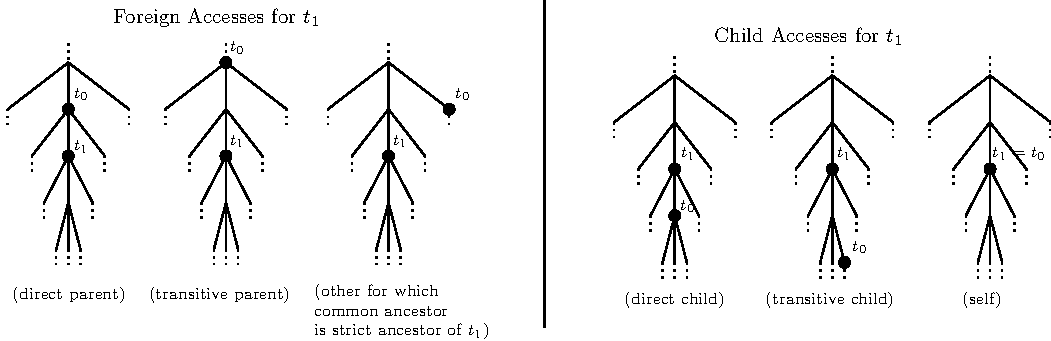
\includegraphics[width=\textwidth]{../figs/accesses-kinds.pdf}
% FIXME: caption

\subsection{Pointer permissions}

\subsubsection{Available permission combinations}

Pointers can have the following permissions:
\begin{itemize}
    \item read permisions: \tperm{Read} or \tperm{!Read};
    \item write permissions: \tperm{Write} or \tperm{Future Write} or \tperm{!Write}.
\end{itemize}

We choose to introduce \tperm{Future Write} permissions as a way for Tree Borrows to
natively handle 2-phase borrows, as is explained in \ref{TODO}.
This does not directly allow write accesses through this pointer, but it reserves
a right to obtain such \tperm{Write} permissions later in the execution.

Tree Borrows uses the following combinations of permissions:
\begin{lstlisting}
enum ReadWritePerms {
    Reserved = Read + Future Write,
    Active = Read + Write,
    Frozen = Read + !Write,
    Disabled = !Read + !Write,
}
\end{lstlisting}

They are to be interpreted in the following way:
\begin{itemize}
    \item a \tperm{Disabled} tag corresponds to a pointer whose lifetime has ended;
    \item a \tperm{Frozen} tag gives read-only permissions to a pointer, so it is suitable
        for shared references without interior mutability;
    \item an \tperm{Active} tag corresponds to a mutable reference that is currently being used mutably;
    \item a \tperm{Reserved} tag corresponds to a mutable reference that has not been used mutably yet.
\end{itemize}

\subsubsection{The purpose of \tperm{Future Write}}

The following code features a so-called ``2-phased borrow'':
\begin{lstlisting}
impl X {
    fn method(&mut self, ...) { ... }
}

x: &mut X
x.method(arg1, arg2, ...);
\end{lstlisting}
where the method call desugars to approximately
\begin{lstlisting}
let x_bor: &mut *x;
                    -----
let arg1 = ...;         |--- special zone within which x is still accessible,
let arg2 = ...;         |    but only immutably
                    -----
X::method(x_bor, arg1, arg2, ...);
\end{lstlisting}
% FIXME: box around the zone

As a concrete example, consider
\begin{lstlisting}
v: &mut Vec<usize>
v.push(v.len());
\end{lstlisting}
which the Borrow Checker accepts despite rejecting the following
\begin{lstlisting}
v: &mut Vec<usize>
let w = &mut *v;
let l = v.len();
Vec::push(w, l);
\end{lstlisting}

Therefore the existence of 2-phase borrows suggests the possibility of a mutable
borrow being ``delayed'': as long as it has not yet been accessed mutably, it still
tolerates shared read-only access. In other words, it does not have a \tperm{Write}
permission yet, but can obtain one in the future. This is exactly how our
\tperm{Future Write} permission is set to behave.

Rather than limiting this behavior to 2-phase borrows only, we choose in Tree
Borrows to make all mutable borrows behave in a uniform way: all mutable references
will wait until their first write access to claim their \tperm{Write} permission,
and will allow shared read-only access in the meantime. If not for this, a lot
of code currently being written would not be accepted, such as some code that
follows the following pattern
\begin{lstlisting}
                             // More generally:
let ptr = vec.as_mut_ptr();  // - some mutable reborrow
if vec.len() > 0 {           // - use base pointer immutably
   do_stuff(ptr)             // - then use the reborrow
}
\end{lstlisting}

A concrete example currently in use in the standard library test suite:
\begin{lstlisting}
let mut x = 2;
let xref = &mut x;
let xraw = &mut *xref as *mut _; // create a mutable reborrow
let xshr = &*xref;
assert_eq!(*xshr, 2); // read-only usage of the base pointer
unsafe {
    *xraw = 4; // usage of the mutable reborrow
}
assert_eq!(x, 4);
\end{lstlisting}

Extending the behavior of 2-phase borrows to all mutable borrows also serves
towards our goal of allowing all reorderings of read-only operations: it lets
us exchange reads through mutable (but not used mutably) references with each
other and with reborrows of other mutable references.

\subsubsection{Initialization}

The initial permissions depend of the type of borrow.
Recall from \ref{TODO} that raw pointers do not receive new permissions and instead
use the same tag and permissions as their parent pointer. This leaves mutable and
shared references for which we must determine an initial permission.

All references obtain a \tperm{Read} permission initially. This is required
because we perform a fake read access upon reborrowing a reference, and it asserts
that all references are dereferenceable (they are tagged \texttt{dereferenceable}
in LLVM).

In addition, mutable references obtain a \tperm{Future Write} permission upon initialization
making them \tperm{Reserved}, while shared references receive \tperm{!Write} which makes them \tperm{Frozen}.

\subsection{Updates}

We now describe how permissions are updated after an access is performed.
The update process is roughly as follows.

In reaction to an access at \tcode{t\tsub{0}}, traverse the tree. For each \tcode{t\tsub{1}} node of the
tree, if \tcode{t\tsub{0}} is a child of \tcode{t\tsub{1}} then the access is a child access at \tcode{t\tsub{1}}; otherwise
it is a foreign access at \tcode{t\tsub{1}}. Based on the type of access (both child/foreign
and read/write) and some local information, determine the new permissions for the
pointer.

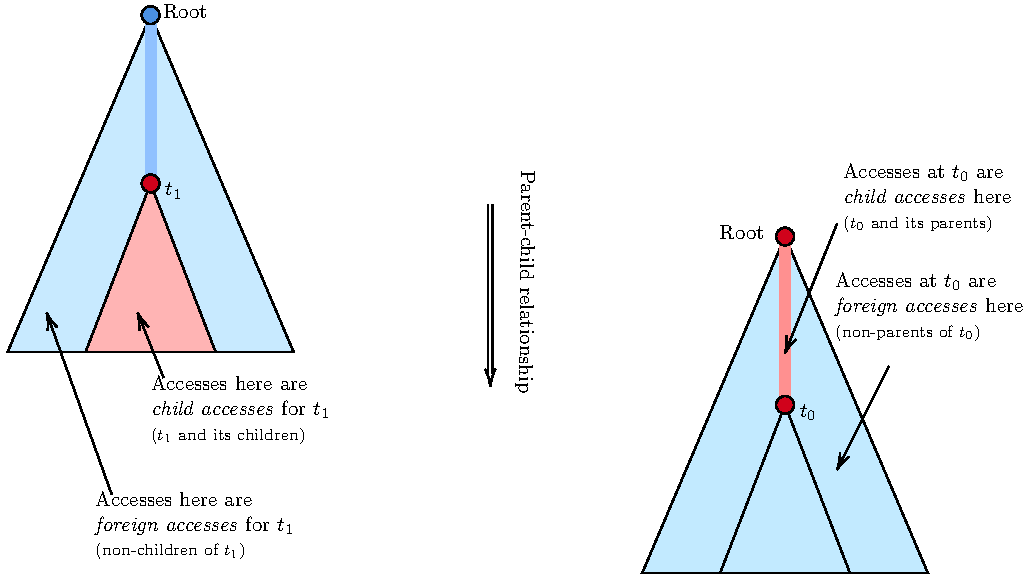
\includegraphics[width=\textwidth]{../figs/child-or-foreign.pdf}
% FIXME: caption

\subsubsection{Intuition on effects of accesses}

\paragraph*{Child accesses}

If \tperm{Active} is to represent mutable references, then it must allow child writes
as well as child reads. Our interpretation of \tperm{Reserved} as a mutable reference
that is not yet used mutably implies that it much be unaffected by child reads,
but turn into \tperm{Active} on the first child write.

\tperm{Frozen} representing a non-interior-mutable shared reference, it must allow
child reads. As child writes are forbidden on such references, we declare any
child write on a \tperm{Frozen} to be UB.

Any child access is obviously UB on a \tperm{Disabled}.

\paragraph*{Foreign accesses on Frozen}

Since shared references allow shared read access, \tperm{Frozen} must be unaffected
by Foreign reads. As shared references on types without interior mutability
assume that no other reference accesses the same data mutably, a \tperm{Frozen} must
become \tperm{Disabled} upon a Foreign write.

\paragraph*{Foreign accesses on Active}

Several mutable references cannot coexist with each other or with shared
references, so an \tperm{Active} must not remain \tperm{Active} upon a foreign access.

If another mutable reference is accessed, which corresponds to a foreign write,
then this \tperm{Active} must lose all permissions and become \tperm{Disabled}.

According to the Borrow Checker, an \tperm{Active} loses all permissions on a Foreign read:
\begin{lstlisting}
// Example 3.A.1
fn main() {
    let base = &mut 42u64;
    let rmut = &mut *base;
    // base: Reserved
    // |-- rmut: Reserved
    *rmut += 1; // Child write for both base and rmut
    // base: Active
    // |--  rmut: Active
    let _val = *base; // Child read for base; foreign read for rmut
    // base: Active
    // |-- rmut: ???
    let _val = *rmut; // Compilation error
    // According to the Borrow Checker, rmut is no longer readable
}
\end{lstlisting}

However we want Tree Borrows to be suited for proving the validity of reordering
any two adjacent read accesses, which means in particular that reordering two
reads should not introduce new UB.

The following piece of code is accepted:
\begin{lstlisting}
// Example 3.A.2
fn main() {
    let base = &mut 42u64;
    let rmut = &mut *base;
    // base: Reserved
    // |-- rmut: Reserved
    *rmut += 1; // Child write for both base and rmut
    // base: Active
    // |--  rmut: Active
    let _val = *rmut; // Child read for both base and rmut
    // base: Active
    // |-- rmut: Active
    let _val = *base; // Child read for base; Foreign read for rmut
    // base: Active
    // |-- rmut: ???
}
\end{lstlisting}
but swapping the two last reads from \textit{Example 3.A.2} would produce \textit{Example 3.A.1} above,
which would be UB if \tperm{Active} were to become \tperm{Disabled} on a foreign read.
We thus choose to make \tperm{Active} become \tperm{Frozen} instead, which means that in
both examples above \tperm{???} should be \tperm{Frozen} and UB occurs in neither.

\paragraph*{Foreign accesses on Reserved}

\tperm{Reserved} is a more special case, and its behavior is guided by the following examples:
\begin{lstlisting}
// Example 3.R.1: Foreign read (standard 2-phase borrow example)
// This must not be UB
fn main() {
    let mut x = vec![];
    // x: Reserved
    x.push( // 2-phase borrow starts here for x' implicitly reborrowed from x
        // x: Reserved
        // |-- x': Active
        x.len() // Foreign read for x'
        // After this, x' must still be writeable inside Vec::push
        // thus a Foreign read must not affect Reserved tags.
    );
}
```

\begin{lstlisting}
// Example 3.R.1': Foreign read outside 2-phase borrow
// This is a very common pattern in the standard library, it must NOT be UB.
// This also justifies why we need to use Reserved for all mutable references,
// and not exclusively for 2-phase borrows.
fn main() {
    let mut x = 2;
    let xref = &mut x;
    let xraw = &mut *xref as *mut _;
    let xshr = &*xref;
    // x: Reserved
    // |-- xref: Reserved
    //     |-- xraw: Reserved
    //     |-- xshr: Frozen
    assert_eq!(*xshr, 2); // This is a Foreign read for xref and xraw
    unsafe { *xraw = 4; } // This is a child write for xref and xraw
                          // meaning it must still be writeable at this point,
                          // therefore the above Foreign read must not have turned
                          // them Frozen.
    assert_eq!(x, 4);
}
\end{lstlisting}

\begin{lstlisting}
// Example 3.R.2: Foreign write
// This should be UB
fn main() {
    let mut x = 2;
    let mut xref = &mut x;
    // x: Reserved
    // |-- xref: Reserved
    *x = 3; // Child write for x; Foreign write for xref
    // x: Active
    // |-- xref: ???
    *xref = 4; // If this is not UB then we are able to alternate writes
               // between two references that each claim exclusive access.
               // This is bad, so xref must no longer have write permissions.
               // The data has been mutated, so xref also can't claim shared
               // read-only access. Therefore Foreign writes must make Reserved
               // turn into Disabled, which causes UB in this example as desired.
    *x = 3;
}
\end{lstlisting}

\begin{lstlisting}
// Example 3.R.2': Foreign write with interior mutability
// This must not be UB
fn main() {
    use std::cell::Cell;
    trait Thing: Sized {
        fn do_the_thing(&mut self, _s: ());
    }

    let mut x = Cell::new(1);
    // x: Reserved
    x.do_the_thing({
        // A 2-phase starts here for x' implicitly reborrowed from x
        // x: Reserved
        // |-- x': Reserved
        x.set(3) // This is a Foreign write for x'
        // x: Active
        // |-- x': ???
    })
    impl<T> Thing for Cell<T> {
        fn do_the_thing(&mut self, _s: ()) {
            // Function call starts, x' is implicitly reborrowed into x''
            // x: Active
            // |-- x': ???
            //     |-- x'': Reserved
            self.set(5): // x' must be readable and writeable
                         // This is a child write for x', which means
                         // that x' is now Active and was not previously Disabled
                         // or Frozen. Therefore x' was previously still Reserved,
                         // even though it was subjected to a Foreign write.
        }
    }
}
\end{lstlisting}

\paragraph*{Ordering of states}

From the above we can observe that all transitions follow the order
\tperm{Reserved < Active < Frozen < Disabled}, which corresponds to the permissions
during a "normal" lifetime of a mutable reference: it is \tperm{Reserved} upon creation
to accomodate for 2-phase borrows, then eventually becomes \tperm{Active} on the first
child write. The next Foreign read marks the end of its period of exclusive access
and it can now only be accessed immutably by becoming \tperm{Frozen}. Eventually its
lifetime ends altogether as a different branch claims exclusive access, it
becomes \tperm{Disabled} and will remain so forever.

\subsubsection{Automata of Permissions}

The full automata of how permissions react to accesses can be seen in \ref{TODO}.
For now this is nothing more than the aggregation of everything established in \ref{TODO}.

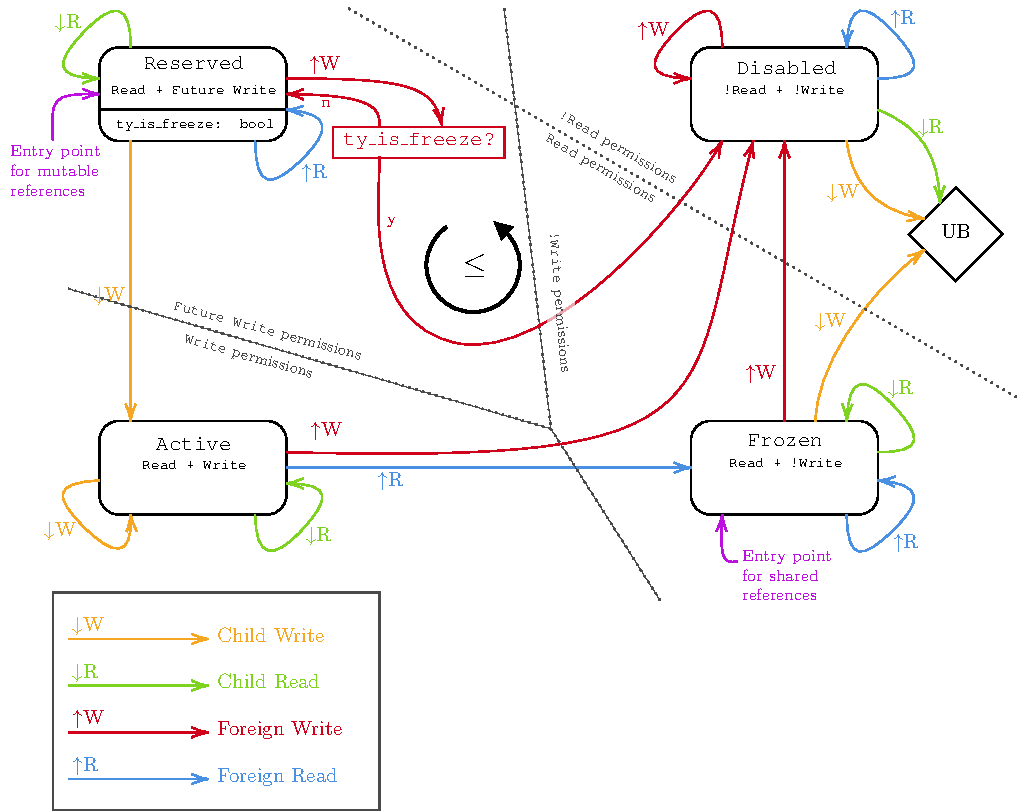
\includegraphics[width=\textwidth]{../figs/state-machine_noprotect.pdf}
% FIXME: caption

A possible interpretation of these transitions:
\begin{itemize}
    \item in reaction to a child access, the state will advance forward according to \tperm{<} until
        it has obtained the required read or write permissions for the access to be performed
        \begin{itemize}
            \item \tperm{Reserved}, \tperm{Active}, and \tperm{Frozen} already have their \tperm{Read} permissions,
                so a child read does not affect them;
            \item \tperm{Active} also has \tperm{Write} permissions, so it is unaffected child Write;
            \item \tperm{Reserved} does not have \tperm{Write} (only \tperm{Future write}), but it can advance to \tperm{Active} to
                obtain the missing permission;
            \item \tperm{Frozen} for a \tperm{Write} and \tperm{Disabled} for both \tperm{Read} and \tperm{Write} have no way of
                obtaining the required permissions, since all reachable states are also missing these
                permissions, this produces UB.
        \end{itemize}
    \item in reaction to a Foreign access, the state will advance forward according to \tcode{<} until
        it has lost the incompatible permissions
        \begin{itemize}
            \item \tperm{Disabled} having no permissions to lose, it has both many looping transitions and many incoming transitions;
            \item \tperm{Frozen} is the destination for an \tperm{Active} that needs to lose its \tperm{Write} permission;
            \item \tperm{Frozen}'s \tperm{!Write} and \tperm{Reserved}'s \tperm{Future Write} are compatible with a Foreign read, hence the loops;
            \item as a unique exception to everything being incompatible with a Foreign write, a \tperm{Reserved} can stay
                \tperm{Reserved} if it has interior mutability, as explained previously by \textit{Example 3.R.2'}.
        \end{itemize}
\end{itemize}

In addition, notice that every state that has an incoming transition for any kind of
access also has a loop to itself for the same kind of access. For example a Foreign read
access on \tperm{Active} leads to \tperm{Frozen}, which is stable under Foreign reads. Similarly
a child write on Reserved leads to \tperm{Active} which is stable under child writes.
This observation is an easy consequence of the "advance until permissions are compatible"
interpretation of the transitions: once a state has been reached with compatible
permissions, applying the same access again will be a no-op because the state
is obviously already compatible. This idempotency of all accesses opens the door
for optimizations: if the consequences of a certain kind of access have already
been applied to some subtree of the borrow tree, said subtree can be skipped entirely
from the tree traversal if the next access is also of the same kind.


\subsubsection{Protectors}

The compiler optimizations that Tree Borrows should justify include LLVM optimizations,
thus Tree Borrows must not allow violations of assumptions made by LLVM. Among these
assumptions is \tcode{noalias} which specifies to what extent a pointer passed as an
argument to a function aliases with other pointers. In Rust, mutable and shared
references are both marked \tcode{noalias}.

% FIXME: quote
\begin{indent}
    \tcode{noalias}

    \begin{indent}
        This indicates that memory locations accessed via pointer values based on the argument
        are not also accessed, during the execution of the function, via pointer values not based on
        the argument. This guarantee only holds for memory locations that are modified,
        by any means, during the execution of the function.
    \end{indent}

    --- from the \href{https://llvm.org/docs/LangRef.html}{LLVM Language Reference Manual}
\end{indent}

This can be reworded in language closer to Tree Borrows:

\begin{indent}
An access via pointer values based on the argument is a child access.
An access via pointer values *not* based on the argument is a Foreign access.
If a tag is marked noalias then during the execution of the function there must
not be both child and Foreign accesses for this tag if at least one of them is a write access.
\end{indent}

This means that the following pieces of code must be Undefined Behavior,
but with the current model not all of them are:
\begin{lstlisting}
// Example 3.N.1
fn main() {
    let data = &mut 42u64;
    let y = data as *const u64;
    let x = &mut *data;
    foreign_read_before_write(x, y);
    fn foreign_read_before_write(x: &mut u64, y: *const u64) {
        // x: Reserved [noalias]
        let _ = unsafe { *y }; // Foreign read for x
        // x: Reserved [noalias]
        *x += 1; // Child write for x
        // /!\ Combined with the previous Foreign read this is a noalias violation
        // x: Active [noalias]
        // -- UB must occur before this point --
        // (With the current model no UB occurs)
    }
}
\end{lstlisting}
\begin{lstlisting}
// Example 3.N.2
fn main() {
    let data = &mut 42u64;
    let y = data as *const u64;
    let x = &mut *data;
    write_before_foreign_read(x, y);
    fn write_before_foreign_read(x: &mut u64, y: *const u64) {
        // x: Reserved [noalias]
        *x += 1; // Child write for x
        // x: Active [noalias]
        let _ = unsafe { *y }; // Foreign read for x
        // /!\ Combined with the previous child write this is a noalias violation
        // x: Frozen [noalias]
        // -- UB must occur before this point --
        // (With the current model no UB occurs)
    }
}
\end{lstlisting}
\begin{lstlisting}
// Example 3.N.3
fn main() {
    let data = &mut 42u64;
    let y = data as *mut u64;
    let x = &*data;
    foreign_write_before_read(x, y);
    fn foreign_write_before_read(x: &u64, y: *mut u64) {
        // x: Frozen [noalias]
        unsafe { *y += 1; } // Foreign write for x
        // x: Disabled [noalias]
        let _ = *x; // Child read for x which has !Write
        // /!\ Combined with the previous Foreign write this is a noalias violation
        // This is already (correctly) UB in the current model
        // -- UB must occur before this point --
    }
}
\end{lstlisting}
\begin{lstlisting}
// Example 3.N.4
fn main() {
    let data = &mut 42u64;
    let y = data as *mut u64;
    let x = &*data;
    read_before_foreign_write(x, y);
    fn read_before_foreign_write(x: &u64, y: *mut u64) {
        // x: Frozen [noalias]
        let _ = *x; // Child read for x
        // x: Frozen [noalias]
        unsafe { *y += 1; } // Foreign write for x
        // /!\ Combined with the previous child read this is a noalias violation
        // x: Disabled [noalias]
        // -- UB must occur before this point --
        // (With the current model no UB occurs)
    }
}
\end{lstlisting}

Only in \textit{Example 3.N.3} is there indeed UB. Here is what the other examples teach
us:

\begin{itemize}
    \item (\textit{Example 3.N.4}) a \tperm{Frozen} becoming \tperm{Disabled} indicates the presence of a
        Foreign write (only possible cause of the transition). If the location was also accessed
        through any child access, then these two accesses violate \tcode{noalias}, thus a transition
        \tperm{Frozen -> Disabled} should be UB on any accessed location;
    \item the same remark applies to a \tperm{Reserved} or \tperm{Active} becoming \tperm{Disabled};
    \item (\textit{Example 3.N.2}) an \tperm{Active} becoming \tperm{Frozen} indicates the presence of a child write
        (requirement for the existence of an \texttt{Active}) and a Foreign write (only possible cause
        of the transition). These two accesses violate \tcode{noalias}, thus a transition \tperm{Active -> Frozen}
        should be UB;
    \item (\textit{Example 3.N.1}) after a Foreign read has occured, \tperm{Reserved} must no longer allow
        child writes. We model this by making it \tperm{Frozen}, which means that the next attempted child write
        would be UB;
    \item for the same reason \tperm{Reserved} must not stay \tperm{Reserved} after a Foreign write even
        if it has interior mutability. We declare that under Foreign write, \tperm{Reserved} becomes
        \tperm{Disabled} which means that the next attempted child read or write would be UB.
\end{itemize}

In terms of read and write permissions, this means that compared to the previous
model without protectors, additional UB occurs on any transition that causes
\tperm{Read -> !Read} or \tperm{Write -> !Write}.

Once the function has returned, the pointer is no longer subjected to \tcode{noalias}
and it resumes reacting ``normally'' to accesses.

To handle this new addition to the model we introduce \textit{Protectors}. Upon function
entry, we add a Protector to every reference passed as argument (Implementation:
simply maintain a \tcode{HashSet} containing call ids of functions that have not yet
returned and their reference arguments, and query this set on each transition
to know if this tag's permissions should follow the protected or unprotected
version of the transitions). In order to not declare too much UB, we also add
to each state a boolean field \tcode{accessed}, which is initially \tcode{false} and becomes
\tcode{true} on the first child access.

Being protected thus modifies the behavior of pointers in the way described in \ref{TODO}.

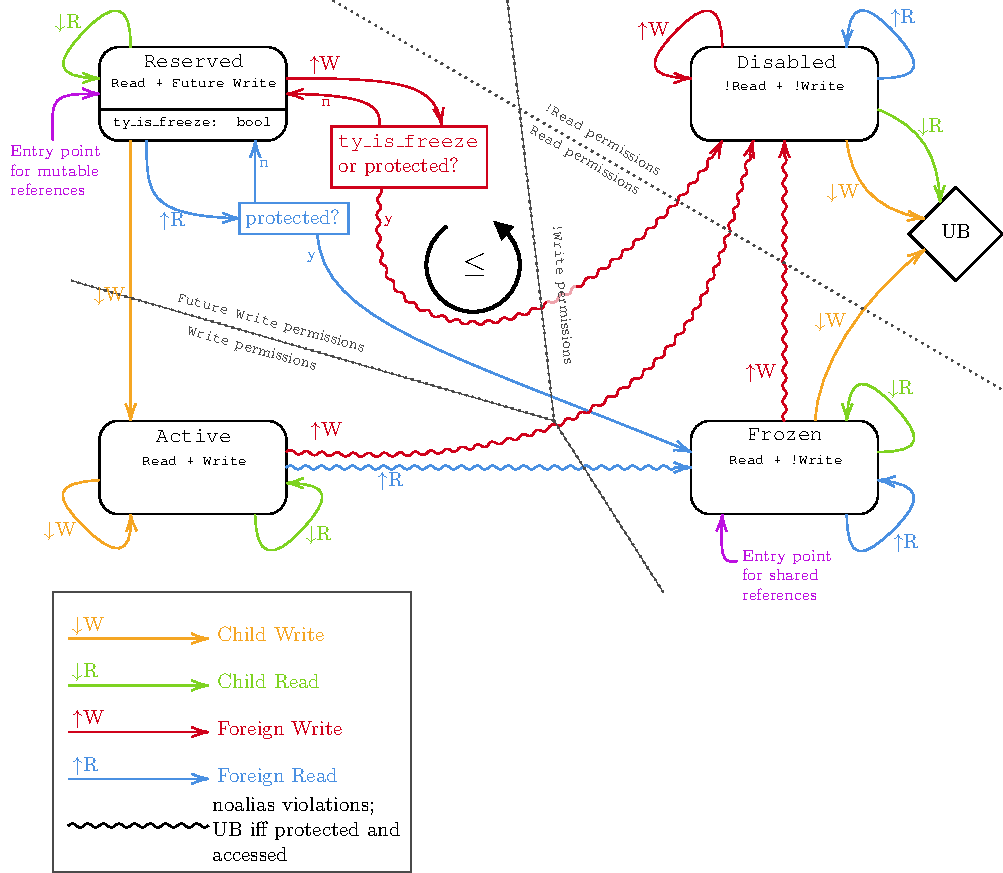
\includegraphics[width=\textwidth]{../figs/state-machine.pdf}
% FIXME: caption

Note: we observed earlier that for every kind of access, the corresponding transitions
are idempotent. The only transitions that have changed and could violate the observation would be

\begin{itemize}
    \item \tperm{Reserved -<foreign read>-> Reserved -<foreign read + protected>-> Frozen}, and
    \item \tperm{Reserved -<foreign write>-> Reserved -<foreign write + protected>-> Disabled},
\end{itemize}

but for these to happen would require that a protector be added after the tag has already been
subjected to an access, which is not something that occurs in our model.
We can thus still rely on the effect of every access being idempotent.

\subsubsection{Accesses outside of initial range}

Tree Borrows is capable of handling pointers with unknown size as well as using
a pointer to access data outside of the range it was reborrowed for.

One such case is
\begin{lstlisting}
fn access_after_offset() { unsafe {
    let data: [u64; 2] = [0, 1];
    let fst = &mut data[0] as *mut u64;
    let snd = fst.add(1);
    ptr::swap(fst, snd);
} }
\end{lstlisting}
Here the reborrow for \tcode{fst} only covers \tcode{data[0]}, but \tcode{snd} is then derived from
\tcode{fst} and translated outside of its original range. As we still wish to check
that even for these accesses no aliasing assumptions are violated, we track
permissions even for locations outside of the range of the initial reborrow.

These permissions outside the range can be initialized lazily rather than as soon
as the reborrow occurs, because it is costly to immediately add permissions
on the entire allocation when they will most likely never be actually used by
a child access.

We do not perform a read access on reborrow for locations outside of the range.

\subsubsection{On whether to propagate loss of permissions}

Consider the following pattern:
\begin{lstlisting}
let x = &mut 42u64;
// x: Reserved
let y = &mut *x; // Child read for x
// x: Reserved
// |-- y: Reserved
*y += 1; // Child write for x and y
// x: Active
// |-- y: Active
let z = &mut *y; // Child read for x and y
// x: Active
// |-- y: Active
//     |-- z: Reserved
let _ = *x; // Child read for x; Foreign read for y and z
// The above setup produces the following tree:
// x: Active
// |-- y: Frozen
//     |-- z: Reserved
\end{lstlisting}
No UB occurs here, the model thus allows having in the tree a \tperm{Frozen} parent with a \tperm{Reserved} child.
This looks like we have derived a mutable reference from a shared reference, which would
be worrying.

We could resolve this concern by making \tcode{z} \tperm{Frozen} as well (i.e. requiring
children of \tperm{Frozen} to be at least \tperm{Frozen} and children of \tperm{Disabled} to be
at least \tperm{Disabled}), but in fact this would result in exactly the same
UB as in the current model and thus non-\tperm{Frozen} children of \tperm{Frozen} are not
a concern.

Indeed from the point of view of child accesses, \tcode{z} has already in practice lost
its \tperm{Write} permission, since any child write for \tcode{z} is also a child write for
\tcode{y} and is thus UB.

Even with the addition of Protectors, and child accesses no longer being the only
kind of accesses that can cause UB, we can observe that the above pattern can
only occur when the tag is unprotected.

Thus not propagating loss of permissions from parents to children (not forcing \tperm{Frozen}
parents to also have \tperm{Frozen} children) can make pointers have more permissions in
appearance (what their \tcode{ReadWritePerms} suggest) than they actually do (what
accesses would cause UB), but never in a way that would affect detection of UB.

\subsection{Summary}

\paragraph*{When creating a new pointer \tcode{z} from an existing \tcode{y}}
\begin{itemize}
    \item if \tcode{z} is a \tcode{Unpin} mutable reference
        \begin{itemize}
            \item perform the effects of a read access through \tcode{y}
            \item add a new child of \tcode{y} in the tree
            \item give it the permissions \tperm{Reserved = Read + Future Write}
            \item keep track of whether it has interior mutability or not
        \end{itemize}
    \item if \tcode{z} is a non-interior-mutable shared reference
        \begin{itemize}
            \item perform the effects of a read access through \tcode{y}
            \item add a new child of \tcode{y} in the tree
            \item give it the permissions \tperm{Frozen = Read + !Write}
        \end{itemize}
    \item otherwise give \tcode{z} the same tag as \tcode{y}, they are indistinguishable from now on
\end{itemize}

\paragraph*{When reading through a pointer \tcode{y}}
\begin{itemize}
    \item for all ancestors \tcode{x} of \tcode{y} (including \tcode{y}), this is a child read
        \begin{itemize}
            \item assert that \tcode{x} has \tperm{Read} (i.e. is \tperm{Frozen} or \tperm{Reserved} or \tperm{Active})
            \item otherwise (if \tcode{x} is \tperm{Disabled}) this is UB
        \end{itemize}
    \item for all non-ancestors \tcode{z} of \tcode{y} (excluding \tcode{y}), this is a foreign read
        \begin{itemize}
            \item turn \tperm{Write} into \tperm{!Write} (i.e. \tperm{Active -> Frozen}); this is UB if \tcode{z} is protected
            \item if \tcode{z} is protected, turn \tperm{Future Write} into \tperm{!Write} (i.e. \tperm{Reserved -> Frozen})
        \end{itemize}
\end{itemize}

\paragraph*{When writing through a pointer \tcode{y}}
\begin{itemize}
    \item for all ancestors \tcode{x} of \tcode{y} (including \texttt{y}), this is a child write
        \begin{itemize}
            \item turn \tperm{Future Write} into \tperm{Write} (i.e. \tperm{Reserved -> Active})
            \item it is UB to encounter \tperm{!Write} (either \tperm{Disabled} or \tperm{Frozen})
        \end{itemize}
    \item for all non-ancestors \tcode{z} of \tcode{y} (excluding \tcode{y}), this is a foreign write
        \begin{itemize}
            \item if \tcode{z} is protected this is always UB; otherwise
            \item if \tcode{z} is \tperm{Reserved} and has interior mutability it is unchanged; otherwise
            \item turn \tperm{Write} and `Future Write` into \tperm{!Write} as well as \tperm{Read} into \tperm{!Read}
                (i.e. \tperm{Reserved -> Disabled} and \tperm{Active -> Disabled})
        \end{itemize}
\end{itemize}


\section{Tree Borrows implemented}

\subsection{Testing the Rust Standard Library}

We used the method described in
\href{https://github.com/rust-lang/miri-test-stdlib}{\texttt{github:rust-lang/miri-test-stdlib}}
to evaluate on the Standard Library that Tree Borrows does not declare "too much UB",
in other words that the code that is currently in use is not considered UB according
to Tree Borrows.

We found two tests that were rejected by Tree Borrows, both were instances of the
following pattern:
\begin{lstlisting}
let mut root = 6u8;        // Base pointer: Active
let mref = &mut root;      // Direct child: Reserved
let ptr = mref as *mut u8; // Uses the same tag as mref
// Write to ptr makes it Active
*ptr = 0;
// Parent read from the point of view of ptr makes it Frozen
assert_eq!(root, 0);
// Attempted write is rejected because Frozen forbids writes
*ptr = 0;
\end{lstlisting}

This pattern was previously accepted by Stacked Borrows, but has now been determined
to be arguably a violation of uniqueness that should not have been accepted in the
first place as well as easy to patch. The fix (which simply consists of
replacing \texttt{\&mut root} with \texttt{addr\_of\_mut!(root)}) was accepted
in \href{https://github.com/rust-lang/rust/pull/107954}{github:rust-lang/rust/pull/107954}.


Other widely used libraries such as \texttt{rand} and \texttt{tokio} already
satisfy the requirements of Tree Borrows, suggesting that most codebases will
need few to no changes if they are to enforce the Tree Borrows semantics.

\subsection{Performance concerns and optimizations}

Tree Borrows is slower than Stacked Borrows.

The semantics require that on every access, every tag of the allocation have its
permissions updated on the corresponding range. On allocations with many reborrows
this can easily lead to a naive implementation of Tree Borrows being slower than
Stacked Borrows by an arbitrarily large multiplicative factor.


Fortunately Tree Borrows has access to easy optimizations that allow it to have
an execution time in the same order of magnitude as that of Stacked Borrows on
realistic code samples. We observe that in practice the slowdown from Stacked Borrows
to Tree Borrows is mostly less than x2 on benchmarks that are specifically designed
to stress the borrow tracker, and about x1.3 on general tests that don't particularly attempt to
push the borrow tracker to its limits.

Note further that the benchmarks that follow compare a very optimized implementation
of Stacked Borrows with a Tree Borrows implementation that was only optimized up to
the point that it would not waste too much time. Fine-tuning the garbage collector
of unused tags and implementing a cache are likely to improve the performance of
Tree Borrows as they have already done for Stacked Borrows.



\begin{tabular}{|l|l|c|c|c|c|}
    \hline
    Project & Test & Runs & SB & TB & Factor \\
    \hline
    \multirow{2}{9em}{Miri}
        & \texttt{slice-get-unchecked} & 5 & 0.56s & 4.15s & {\color{Red}x7.41} \\
        & \texttt{mse} & 5 & 0.67s & 1.42s & {\color{Red}x2.12} \\
        & \texttt{serde1} & 5 & 1.53s & 2.60s & {\color{YellowOrange}x1.70} \\
        & \texttt{serde2} & 5 & 3.19s & 5.16s & {\color{YellowOrange}x1.62} \\
        & \texttt{unicode} & 5 & 1.27s & 1.99s & {\color{YellowOrange}x1.57} \\
        & \texttt{backtraces} & 5 & 4.01s & 5.81s & {\color{YellowOrange}x1.45} \\
    \hline
    \multirow{3}{9em}{Stdlib}
        & \texttt{core} & 1 & 4m31s & 9m15s & {\color{Red}x2.05} \\
        & \texttt{alloc} & 1 & 4m45s & 5m54s & {\color{LimeGreen}x1.24} \\
        & \texttt{std/time} & 1 & 15.1s & 17.5s & {\color{LimeGreen}x1.16} \\
    \hline
    \multirow{1}{9em}{Regex}
        & \texttt{lib} & 1 & 13.3s & 20.6s & {\color{YellowOrange}x1.54} \\
    \multirow{1}{9em}{Hashbrown}
        & \texttt{lib} & 1 & 31.5s & 38.3s & {\color{LimeGreen}x1.21} \\
    \multirow{1}{9em}{Tokio}
        & \texttt{lib} & 1 & 40.7s & 45.3s & {\color{LimeGreen}x1.11} \\
    \multirow{1}{9em}{Rand}
        & \texttt{lib} & 1 & 1m24s & 1m31s & {\color{LimeGreen}x1.08} \\
    \hline
\end{tabular}

\begin{itemize}
    \item Miri
        \begin{description}
            \item[Source] \href{https://github.com/rust-lang/miri}{\texttt{github:rust-lang/miri}}
            \item[Command] \texttt{MIRIFLAGS="" ./miri bench}
        \end{description}
    \item Miri-test-stdlib
        \begin{description}
            \item[Source] \href{https://github.com/rust-lang/miri-test-stdlib}{\texttt{github:rust-lang/miri-test-stdlib}}
            \item[Command] \texttt{MIRIFLAGS="" ./run-test.sh core --lib --tests}
            \item[Command] \texttt{MIRIFLAGS="" ./run-test.sh alloc --lib --tests}
            \item[Command] \texttt{MIRIFLAGS="-Zmiri-disable-isolation"}\\
                \texttt{./run-test.sh std --lib --tests -- time::}
        \end{description}
    \item Tokio
        \begin{description}
            \item[Source] \href{https://github.com/tokio-rs/tokio}{\texttt{github:tokio-rs/tokio}}
            \item[Command] \texttt{MIRIFLAGS="-Zmiri-disable-isolation -Zmiri-tag-raw-pointers"} \\
                \texttt{cargo +nightly miri test --features full --lib}
        \end{description}
    \item Rand
        \begin{description}
            \item[Source] \href{https://github.com/rust-random/rand}{\texttt{github:rust-random/rand}}
            \item[Command] \texttt{MIRIFLAGS="" cargo +nightly miri test --lib}
        \end{description}
    \item Hashbrown
        \begin{description}
            \item[Source] \href{https://github.com/rust-lang/hashbrown}{\texttt{github:rust-lang/hashbrown}}
            \item[Command] \texttt{MIRIFLAGS="" cargo +nightly miri test --lib}
        \end{description}
    \item Regex
        \begin{description}
            \item[Source] \href{https://github.com/rust-lang/regex}{\texttt{github:rust-lang/regex}}
            \item[Command] \texttt{MIRIFLAGS="" cargo +nightly miri test --lib -- --skip encode\_decode}
        \end{description}


\end{itemize}

\section{Future work}

\subsection{Formalization}

\subsection{Proving optimizations}


%%
%% Bibliography
%%
% Rustc dev guide: https://rustc-dev-guide.rust-lang.org/borrow_check/two_phase_borrows.html

\bibliography{literature}


\newpage
\appendix

\end{document}
